\documentclass{beamer}\usepackage[]{graphicx}\usepackage[]{color}
%% maxwidth is the original width if it is less than linewidth
%% otherwise use linewidth (to make sure the graphics do not exceed the margin)
\makeatletter
\def\maxwidth{ %
  \ifdim\Gin@nat@width>\linewidth
    \linewidth
  \else
    \Gin@nat@width
  \fi
}
\makeatother

\definecolor{fgcolor}{rgb}{0.345, 0.345, 0.345}
\newcommand{\hlnum}[1]{\textcolor[rgb]{0.686,0.059,0.569}{#1}}%
\newcommand{\hlstr}[1]{\textcolor[rgb]{0.192,0.494,0.8}{#1}}%
\newcommand{\hlcom}[1]{\textcolor[rgb]{0.678,0.584,0.686}{\textit{#1}}}%
\newcommand{\hlopt}[1]{\textcolor[rgb]{0,0,0}{#1}}%
\newcommand{\hlstd}[1]{\textcolor[rgb]{0.345,0.345,0.345}{#1}}%
\newcommand{\hlkwa}[1]{\textcolor[rgb]{0.161,0.373,0.58}{\textbf{#1}}}%
\newcommand{\hlkwb}[1]{\textcolor[rgb]{0.69,0.353,0.396}{#1}}%
\newcommand{\hlkwc}[1]{\textcolor[rgb]{0.333,0.667,0.333}{#1}}%
\newcommand{\hlkwd}[1]{\textcolor[rgb]{0.737,0.353,0.396}{\textbf{#1}}}%

\usepackage{framed}
\makeatletter
\newenvironment{kframe}{%
 \def\at@end@of@kframe{}%
 \ifinner\ifhmode%
  \def\at@end@of@kframe{\end{minipage}}%
  \begin{minipage}{\columnwidth}%
 \fi\fi%
 \def\FrameCommand##1{\hskip\@totalleftmargin \hskip-\fboxsep
 \colorbox{shadecolor}{##1}\hskip-\fboxsep
     % There is no \\@totalrightmargin, so:
     \hskip-\linewidth \hskip-\@totalleftmargin \hskip\columnwidth}%
 \MakeFramed {\advance\hsize-\width
   \@totalleftmargin\z@ \linewidth\hsize
   \@setminipage}}%
 {\par\unskip\endMakeFramed%
 \at@end@of@kframe}
\makeatother

\definecolor{shadecolor}{rgb}{.97, .97, .97}
\definecolor{messagecolor}{rgb}{0, 0, 0}
\definecolor{warningcolor}{rgb}{1, 0, 1}
\definecolor{errorcolor}{rgb}{1, 0, 0}
\newenvironment{knitrout}{}{} % an empty environment to be redefined in TeX

\usepackage{alltt}

%normal
\usepackage{color}
\usepackage{beamerthemebars}
\usepackage{lmodern}
\usepackage{multicol}
\usepackage{booktabs}



\usetheme{AnnArbor}
\usecolortheme{wolverine}

%redefined colors for beamer
\definecolor{beamer@UIUCblue}{RGB}{0,60,125}
\definecolor{beamer@UIUCorange}{RGB}{244,127,36}
% taken from 
% http://identitystandards.illinois.edu/graphicstandardsmanual/generalguidelines/colors.html

\definecolor{beamer@UIUCgray}{RGB}{210,210,210}
%warning text
\definecolor{customgreen}{RGB}{2,103,1}

\setbeamercolor{frametitle}{fg=beamer@UIUCblue,bg=beamer@UIUCgray}
\setbeamercolor{normal text}{fg=black}
\setbeamercolor{title}{fg=beamer@UIUCblue,bg=beamer@UIUCorange}
\setbeamercolor{item projected}{fg=white,bg=beamer@UIUCorange}
%boxes
\setbeamercolor{block title}{fg=beamer@UIUCblue,bg=beamer@UIUCorange}
\setbeamercolor{block body}{fg=blue,bg=beamer@UIUCblue!80}
\setbeamercolor{title in head/foot}{fg=beamer@UIUCblue,bg=beamer@UIUCgray}
\setbeamercolor{author in head/foot}{fg=white,bg=beamer@UIUCblue}
\setbeamercolor{institute in head/foot}{fg=white,bg=beamer@UIUCorange}
\setbeamercolor{date in head/foot}{fg=white,bg=beamer@UIUCorange}
\setbeamercolor{section in head/foot}{fg=white,bg=beamer@UIUCblue}
\setbeamercolor{subsection in head/foot}{fg=white,bg=beamer@UIUCorange}

%override title link color
\makeatletter
\renewcommand\insertshorttitle[1][]{%
  \beamer@setupshort{#1}%
  \let\thanks=\@gobble%
  \ifnum\c@page=1%
  \hyperlinkpresentationend{\beamer@insertshort{\usebeamercolor*[fg]{title in head/foot}\beamer@shorttitle}}%
  \else%
  \hyperlinkpresentationstart{\beamer@insertshort{\usebeamercolor*[fg]{title in head/foot}\beamer@shorttitle}}%
  \fi}
\makeatother

\usepackage{etoolbox}
\makeatletter
\patchcmd{\beamer@section}
  {\def\insertsectionhead{\hyperlink{Navigation\the\c@page}{#1}}}
  {\def\insertsectionhead{\hyperlink{Navigation\the\c@page}{\usebeamercolor*[fg]{section in head/foot}#1}}}
  {}{}
\patchcmd{\beamer@subsection}
  {\def\insertsubsectionhead{\hyperlink{Navigation\the\c@page}{#1}}}
  {\def\insertsubsectionhead{\hyperlink{Navigation\the\c@page}{\usebeamercolor*[fg]{subsection in head/foot}#1}}}
  {}{}
\makeatother


%insert timeline
\AtBeginSection[]
{
  \begin{frame}
    \frametitle{On the Agenda}
    \begin{multicols}{2}
    \tableofcontents[currentsection]
    \end{multicols}
  \end{frame}
}


%\setbeamercolor{palette tertiary}{bg=beamer@UIUCblue,fg=white}
%\setbeamercolor{palette secondary}{bg=beamer@UIUCgray,fg=white}
%\setbeamercolor{palette primary}{bg=beamer@UIUCorange,fg=white}

\beamertemplatenavigationsymbolsempty %hides navigation.
\usepackage{graphicx}
\usepackage{comment}
\usepackage{hyperref}
\hypersetup{colorlinks=true,urlcolor=beamer@UIUCblue,linkcolor=beamer@UIUCblue,% link color controls section, subsection, and title
citecolor = beamer@UIUCorange,
anchorcolor = beamer@UIUCorange}
\usepackage{amssymb,amsmath}
\usepackage{multirow}
\usepackage{upgreek}

%flow charts
\usepackage{tikz}
\usetikzlibrary{shapes,arrows,positioning}

\author[J Balamuta]{James Balamuta}
\institute[UIUC]{Department of Statistics \\
University of Illinois at Urbana-Champaign \\
\href{mailto:balamut2@illinois.edu}{\nolinkurl{balamut2@illinois.edu} }}





\IfFileExists{upquote.sty}{\usepackage{upquote}}{}
\begin{document}


\date[STAT 385]{June 13, 2016 \\ Summer Session 2 - 2016}

\title[Course Introduction]{
\begin{columns}
\column{.15\textwidth}
\hspace{.2in}
\vspace{.1in}

\includegraphics{imark_bold-eps-converted-to.pdf}
\column{.85\textwidth}
{STAT 385: Statistics Programming Methods}
\end{columns}
}
\frame{\titlepage}

\begin{frame}
\frametitle{On the Agenda}   
\begin{multicols}{2}
\tableofcontents[]
\end{multicols}
\end{frame}


\section{Intro}
\subsection{Profiles}

\begin{frame}
\begin{center}
\makeatletter

\pgfkeys{/pgf/.cd,
  rectangle corner radius north west/.initial=10pt,
  rectangle corner radius north east/.initial=10pt,
  rectangle corner radius south west/.initial=10pt,
  rectangle corner radius south east/.initial=10pt
}
\newif\ifpgf@rectanglewrc@donecorner@
\def\pgf@rectanglewithroundedcorners@docorner#1#2#3#4#5{%
  \edef\pgf@marshal{%
    \noexpand\pgfintersectionofpaths
      {%
        \noexpand\pgfpathmoveto{\noexpand\pgfpoint{\the\pgf@xa}{\the\pgf@ya}}%
        \noexpand\pgfpathlineto{\noexpand\pgfpoint{\the\pgf@x}{\the\pgf@y}}%
      }%
      {%
        \noexpand\pgfpathmoveto{\noexpand\pgfpointadd
          {\noexpand\pgfpoint{\the\pgf@xc}{\the\pgf@yc}}%
          {\noexpand\pgfpoint{#1}{#2}}}%
        \noexpand\pgfpatharc{#3}{#4}{#5}%
      }%
    }%
  \pgf@process{\pgf@marshal\pgfpointintersectionsolution{1}}%
  \pgf@process{\pgftransforminvert\pgfpointtransformed{}}%
  \pgf@rectanglewrc@donecorner@true
}
\pgfdeclareshape{rectangle with rounded corners}
{
  \inheritsavedanchors[from=rectangle] % this is nearly a rectangle
  \inheritanchor[from=rectangle]{north}
  \inheritanchor[from=rectangle]{north west}
  \inheritanchor[from=rectangle]{north east}
  \inheritanchor[from=rectangle]{center}
  \inheritanchor[from=rectangle]{west}
  \inheritanchor[from=rectangle]{east}
  \inheritanchor[from=rectangle]{mid}
  \inheritanchor[from=rectangle]{mid west}
  \inheritanchor[from=rectangle]{mid east}
  \inheritanchor[from=rectangle]{base}
  \inheritanchor[from=rectangle]{base west}
  \inheritanchor[from=rectangle]{base east}
  \inheritanchor[from=rectangle]{south}
  \inheritanchor[from=rectangle]{south west}
  \inheritanchor[from=rectangle]{south east}

  \savedmacro\cornerradiusnw{%
    \edef\cornerradiusnw{\pgfkeysvalueof{/pgf/rectangle corner radius north west}}%
  }
  \savedmacro\cornerradiusne{%
    \edef\cornerradiusne{\pgfkeysvalueof{/pgf/rectangle corner radius north east}}%
  }
  \savedmacro\cornerradiussw{%
    \edef\cornerradiussw{\pgfkeysvalueof{/pgf/rectangle corner radius south west}}%
  }
  \savedmacro\cornerradiusse{%
    \edef\cornerradiusse{\pgfkeysvalueof{/pgf/rectangle corner radius south east}}%
  }

  \backgroundpath{%
    \northeast\advance\pgf@y-\cornerradiusne\relax
    \pgfpathmoveto{}%
    \pgfpatharc{0}{90}{\cornerradiusne}%
    \northeast\pgf@ya=\pgf@y\southwest\advance\pgf@x\cornerradiusnw\relax\pgf@y=\pgf@ya
    \pgfpathlineto{}%
    \pgfpatharc{90}{180}{\cornerradiusnw}%
    \southwest\advance\pgf@y\cornerradiussw\relax
    \pgfpathlineto{}%
    \pgfpatharc{180}{270}{\cornerradiussw}%
    \northeast\pgf@xa=\pgf@x\advance\pgf@xa-\cornerradiussw\southwest\pgf@x=\pgf@xa
    \pgfpathlineto{}%
    \pgfpatharc{270}{360}{\cornerradiusse}%
    %\northeast\advance\pgf@y-\cornerradiusse\relax
    \northeast\advance\pgf@y-\cornerradiusne\relax
    \pgfpathlineto{}%

  }

  \anchor{before north east}{\northeast\advance\pgf@y-\cornerradiusne}
  \anchor{after north east}{\northeast\advance\pgf@x-\cornerradiusne}
  \anchor{before north west}{\southwest\pgf@xa=\pgf@x\advance\pgf@xa\cornerradiusnw
    \northeast\pgf@x=\pgf@xa}
  \anchor{after north west}{\northeast\pgf@ya=\pgf@y\advance\pgf@ya-\cornerradiusnw
    \southwest\pgf@y=\pgf@ya}
  \anchor{before south west}{\southwest\advance\pgf@y\cornerradiussw}
  \anchor{after south west}{\southwest\advance\pgf@x\cornerradiussw}
  \anchor{before south east}{\northeast\pgf@xa=\pgf@x\advance\pgf@xa-\cornerradiusse
    \southwest\pgf@x=\pgf@xa}
  \anchor{after south east}{\southwest\pgf@ya=\pgf@y\advance\pgf@ya\cornerradiusse
    \northeast\pgf@y=\pgf@ya}

  \anchorborder{%
    \pgf@xb=\pgf@x% xb/yb is target
    \pgf@yb=\pgf@y%
    \southwest%
    \pgf@xa=\pgf@x% xa/ya is se
    \pgf@ya=\pgf@y%
    \northeast%
    \advance\pgf@x by-\pgf@xa%
    \advance\pgf@y by-\pgf@ya%
    \pgf@xc=.5\pgf@x% x/y is half width/height
    \pgf@yc=.5\pgf@y%
    \advance\pgf@xa by\pgf@xc% xa/ya becomes center
    \advance\pgf@ya by\pgf@yc%
    \edef\pgf@marshal{%
      \noexpand\pgfpointborderrectangle
      {\noexpand\pgfqpoint{\the\pgf@xb}{\the\pgf@yb}}
      {\noexpand\pgfqpoint{\the\pgf@xc}{\the\pgf@yc}}%
    }%
    \pgf@process{\pgf@marshal}%
    \advance\pgf@x by\pgf@xa% 
    \advance\pgf@y by\pgf@ya%
    \pgfextract@process\borderpoint{}%
    %
    \pgf@rectanglewrc@donecorner@false
    %
    % do southwest corner
    \southwest\pgf@xc=\pgf@x\pgf@yc=\pgf@y
    \advance\pgf@xc\cornerradiussw\relax\advance\pgf@yc\cornerradiussw\relax 
    \borderpoint
    \ifdim\pgf@x<\pgf@xc\relax\ifdim\pgf@y<\pgf@yc\relax
      \pgf@rectanglewithroundedcorners@docorner{-\cornerradiussw}{0pt}{180}{270}{\cornerradiussw}%
    \fi\fi
    %
    % do southeast corner
    \ifpgf@rectanglewrc@donecorner@\else
      \southwest\pgf@yc=\pgf@y\relax\northeast\pgf@xc=\pgf@x\relax
      \advance\pgf@xc-\cornerradiusse\relax\advance\pgf@yc\cornerradiusse\relax
      \borderpoint
      \ifdim\pgf@x>\pgf@xc\relax\ifdim\pgf@y<\pgf@yc\relax
       \pgf@rectanglewithroundedcorners@docorner{0pt}{-\cornerradiusse}{270}{360}{\cornerradiusse}%
      \fi\fi
    \fi
    %
    % do northeast corner
    \ifpgf@rectanglewrc@donecorner@\else
      \northeast\pgf@xc=\pgf@x\relax\pgf@yc=\pgf@y\relax
      \advance\pgf@xc-\cornerradiusne\relax\advance\pgf@yc-\cornerradiusne\relax
      \borderpoint
      \ifdim\pgf@x>\pgf@xc\relax\ifdim\pgf@y>\pgf@yc\relax
       \pgf@rectanglewithroundedcorners@docorner{\cornerradiusne}{0pt}{0}{90}{\cornerradiusne}%
      \fi\fi
    \fi
    %
    % do northwest corner
    \ifpgf@rectanglewrc@donecorner@\else
      \northeast\pgf@yc=\pgf@y\relax\southwest\pgf@xc=\pgf@x\relax
      \advance\pgf@xc\cornerradiusnw\relax\advance\pgf@yc-\cornerradiusnw\relax
      \borderpoint
      \ifdim\pgf@x<\pgf@xc\relax\ifdim\pgf@y>\pgf@yc\relax
       \pgf@rectanglewithroundedcorners@docorner{0pt}{\cornerradiusnw}{90}{180}{\cornerradiusnw}%
      \fi\fi
    \fi
  }
}

\makeatother

\begin{tikzpicture}[every node/.style={minimum width = 10 cm, minimum height=1cm, text centered, inner sep=0, outer sep=0}]

\fontfamily{pag}{\fontsize{1cm}{1cm}\selectfont
    \node [fill=red, node distance=0pt, text=white,rectangle with rounded corners,rectangle corner radius south west=0pt,rectangle corner radius south east=0pt](A){Hello};
}

\fontfamily{pag}{\fontsize{.65cm}{.65cm}\selectfont
    \node [fill=red, node distance=0pt, text=white, outer sep=.4cm, below=of A.center](B){my name is};
}

\fontfamily{augie}{\fontsize{2.6cm}{1cm}\selectfont
    \node [minimum height = 1.5cm, below=of B, align=center](C){James \\ $ $};
}
    \node [fill=red, node distance=0pt, minimum height = 0.5cm, below=of C, rectangle with rounded corners,rectangle corner radius north west=0pt,rectangle corner radius north east=0pt]{};
\end{tikzpicture}
\end{center}
\end{frame}



\begin{frame}
\frametitle{Who am I?}
  \begin{columns}
    \begin{column}{.39\linewidth}
    \centering
    
    
\includegraphics[width=.5\linewidth]{scuba_diving}
\includegraphics[width=.612\linewidth]{lazer} \\
    
\includegraphics[width=.5675\linewidth]{drone}
    \end{column}
    \begin{column}{.6\linewidth}
      \begin{itemize}
        \item 3rd Year PhD Statistics/Informatics
        \item Research
        \begin{itemize}
          \item NASA Carbon Monitor System Project
          \item Time Series Latent Variable Estimation
          \item Choice in Psychometric Models 
        \end{itemize}
        
        \item Teaching
        \begin{itemize}
          \item List of Excellent Teachers (SU 2014)
          \item Created three courses:
          \begin{itemize}
            \item STAT 330: Data Visualization
            \item STAT 385: Statistics Programming Methods (yes, \textbf{this} course!)
            \item STAT 480: Data Science Foundations
          \end{itemize}
        \end{itemize}
      \end{itemize}
    \end{column}
  \end{columns}
\end{frame}


\begin{frame}[fragile]
\frametitle{You are... }



\begin{knitrout}
\definecolor{shadecolor}{rgb}{0.969, 0.969, 0.969}\color{fgcolor}

{\centering 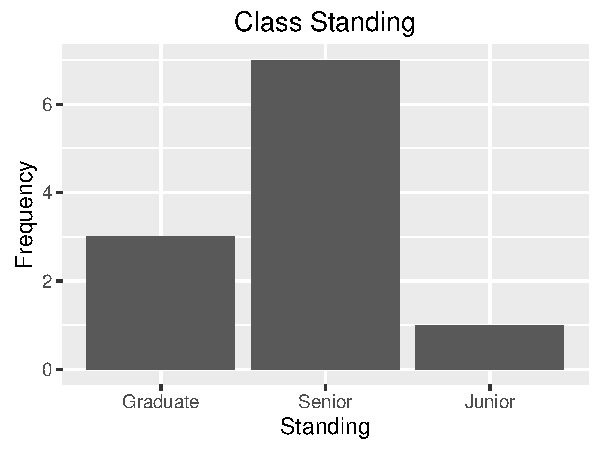
\includegraphics[width=\maxwidth]{figure/enrollment_level-1} 

}



\end{knitrout}

\end{frame}


\begin{frame}[fragile]
\frametitle{You are... }

\begin{knitrout}
\definecolor{shadecolor}{rgb}{0.969, 0.969, 0.969}\color{fgcolor}

{\centering 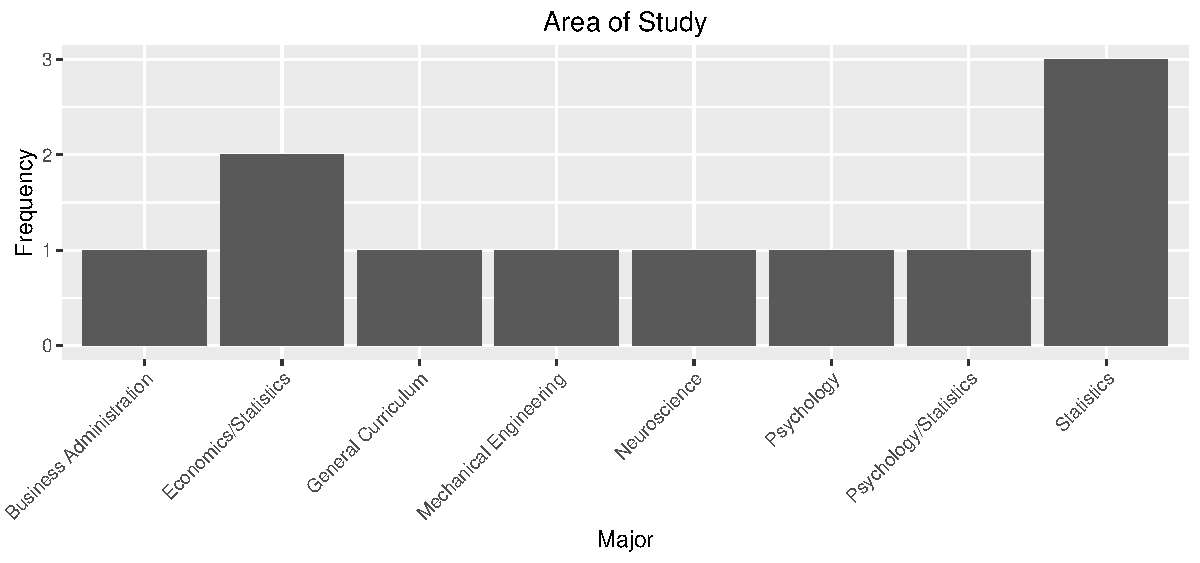
\includegraphics[width=\maxwidth]{figure/enrollment_major-1} 

}



\end{knitrout}

\end{frame}


\begin{frame}[fragile]
\frametitle{Survey says...}

\centering
\Huge
\href{https://docs.google.com/forms/d/1SfdWzg1Ak2ZttHhWRJf1e8vKMbaFzBDT_HVUHyuIO3k/viewanalytics#responses}{Entrance Survey Responses}

\end{frame}

\begin{frame}
\begin{center}
{\fontsize{2.5cm}{2cm}\selectfont{Now you!}}
\\
{\fontsize{1cm}{2cm}\selectfont{What's your name?}}\\$ $\\
{\fontsize{1cm}{2cm}\selectfont{Why are you here?}}
\end{center}
\end{frame}


\subsection{Course Structure}

\begin{frame}
\frametitle{Course Websites}

$ $\\$ $\\$ $\\
\centering
{\Large
Material will be posted to \\$ $\\
\url{http://stat385.thecoatlessprofessor.com/}}
\\$ $\\$ $\\$ $\\$ $\\
\hfill Source code: \url{https://github.com/coatless/stat385/}
\end{frame}

\begin{frame}
\frametitle{Course Websites}

$ $\\$ $\\$ $\\
\centering
{\Large
Discussion and Questions should be posted to \\$ $\\
\url{https://piazza.com/illinois/summer2016/stat385}}
$ $\\$ $\\$ $\\
\centering
{\Large
Online Analytical Environment \\$ $\\
\url{https://rstudio.stat.illinois.edu/}}
\end{frame}

\begin{frame}
\frametitle{About the Course}

\begin{itemize}
\item Emphasize computing theory and methods for statistical algorithms
\item Learn about computing to use in a future career or graduate school
\item Will primarily cover R and C++ (through \href{http://gallery.rcpp.com}{Rcpp})
\end{itemize}

\end{frame}

\begin{frame}
\frametitle{About the Course}

\begin{itemize}
\item Lots of work is ahead of you!
\begin{itemize}
\item Writing code, reading chapters, and working in a group.
\end{itemize}
\item Focus is on creating content rather than consuming it.
\item Lots of open spaces, invite your friends! (Just fill out the \href{https://registrar.illinois.edu/Media/Default/RGSTRNS/Auditors_Permit.pdf}{audit form})
\end{itemize}

\end{frame}


\begin{frame}
\frametitle{Course Objectives}

\begin{itemize}
  \item View different statistical concepts presented from STAT 200 (and select foundational topics from 400-level STAT courses) from a programming perspective instead of a purely theoretical framework.
  \item Implement different statistical algorithm.
  \item \emph{Explain} the underlying algorithm.
  \item Use version control
  \item Distributed computing
  \item Handle a Whiteboard interview
  \item Group capstone project
\end{itemize}

\end{frame}

\begin{frame}
\frametitle{Group Projects}
The group capstone project is meant to showcase the knowledge that you have acquired throughout the course. This is an example that will be invaluable to you when applying for a job or to graduate school. 

\begin{itemize}
\item Defines your experience in this course;
\item Must be fully functional;
\item Choose groups carefully!
\end{itemize}

\end{frame}

\begin{frame}
\frametitle{Types of Projects}
\begin{itemize}
\item Changes pre-existing functions in a statistical package
\item Enables \emph{new} features in a statistical computing environment
\item You pick!
\begin{itemize}
\item Graphics? Fantasy Sports Reader? Grading Application? 
\end{itemize}
\end{itemize}
\end{frame}

\begin{frame}
\frametitle{Point Distribution}

\begin{table}
\centering
\begin{tabular}{lcc}
\toprule
Type & Points Per & Total Points\\ \midrule
Participation & 25 & 25  \\ 
Homework & $8 \times 25$  & 200  \\
Exam & 125 & 125 \\ 
Group Project & $4 \times 37.5$  & 150  \\ \bottomrule
Course Total &  & 500 \\ 
\end{tabular}
\caption{Course Point Distribution}
\label{tab:course}
\end{table}

\end{frame}



\begin{frame}
\frametitle{One last thing...}

This course has been made possible by the encouragement, understanding (of the many errors), and enthusiasm from the following folks:

\Huge{
\begin{itemize}
\item Prof. Jeffrey Douglas
\item Dr. Alexey Stepanov
\item Prof. Steven Culpepper
\item Prof. Douglas Simpson
\item Prof. Stephane Guerrier
\end{itemize}
}

\center \huge Thank you!

\end{frame}


\section{Intro to Programming}

\subsection{Motivation}

\begin{frame}
\frametitle{Age Old Question}

\begin{columns}
\begin{column}{0.5\textwidth}
    \begin{center}
     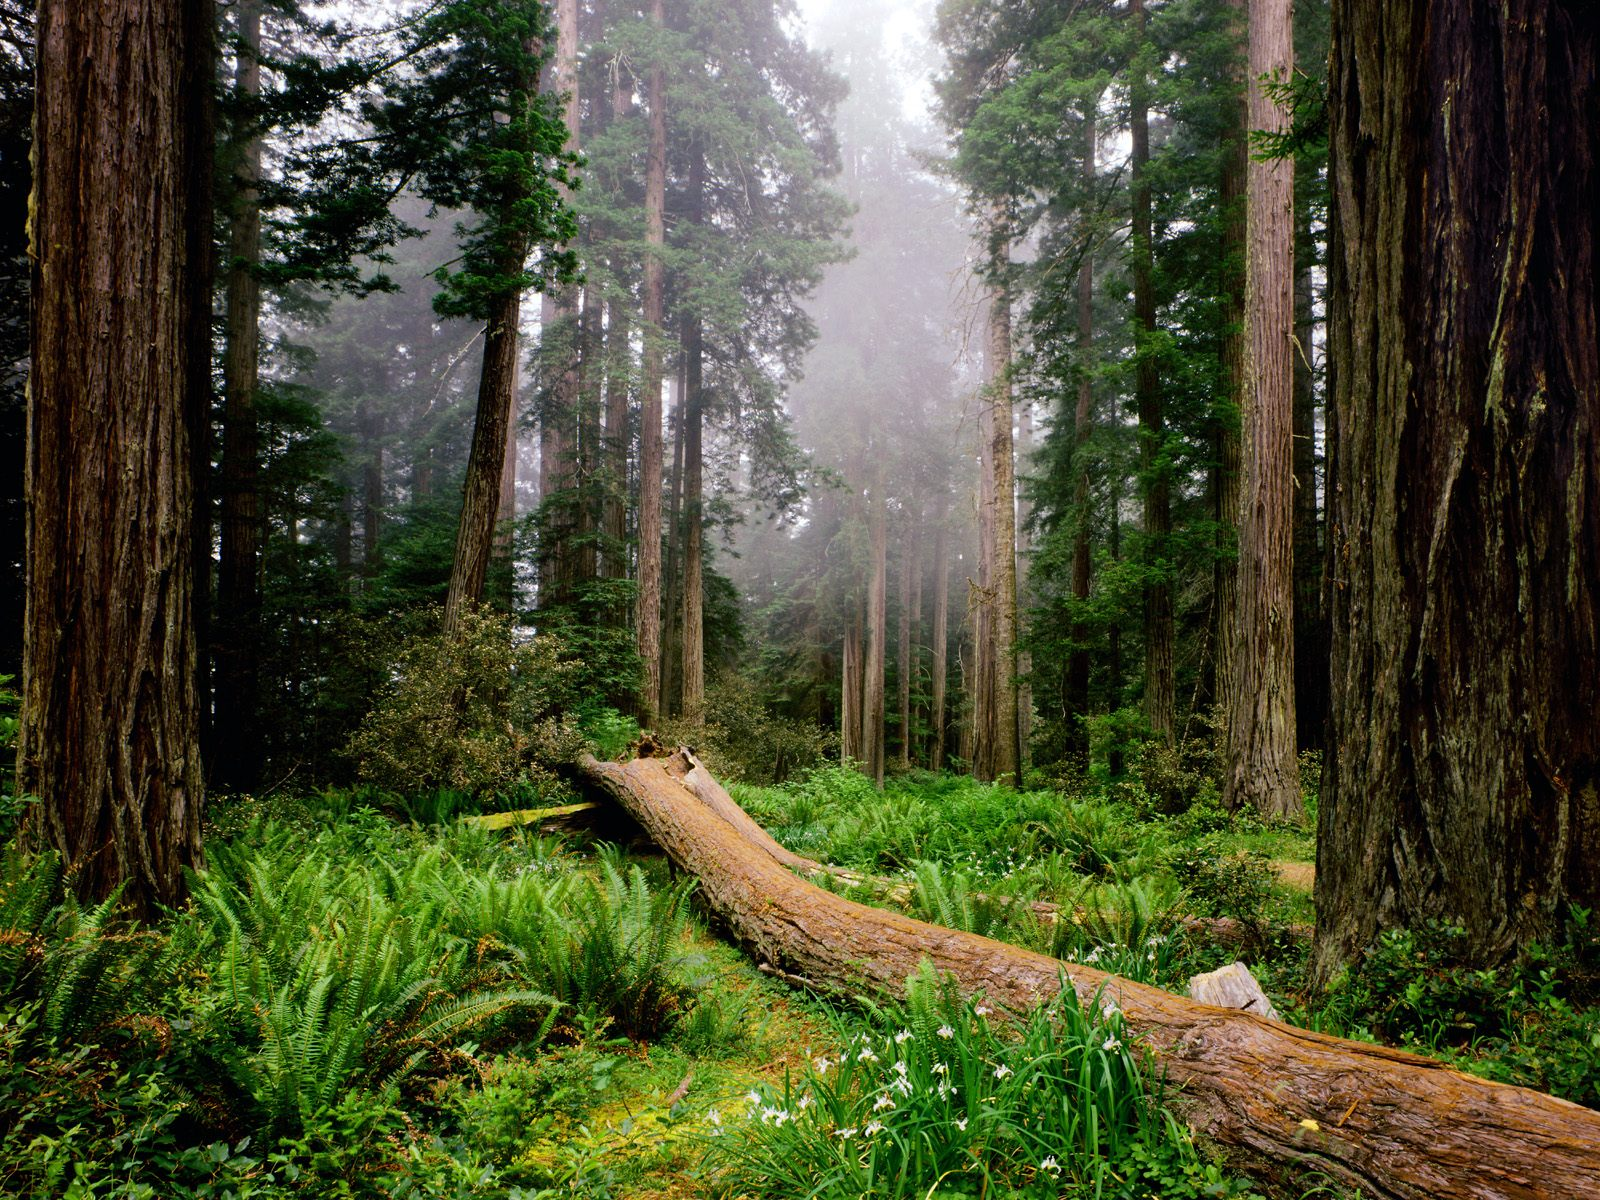
\includegraphics[width=0.85\textwidth]{fallen_tree_in_forest}
     \end{center}
\end{column}
\begin{column}{0.5\textwidth}  %%<--- here

``If a tree falls in a forest and no one is around to hear it, does it make a sound?''

\end{column}
\end{columns}

\end{frame}


\begin{frame}
\frametitle{Age Old Question Redux}

Original: \\$ $\\
{\Large
``If a tree falls in a forest and no one is around to hear it, does it make a sound?''
}
\\$ $\\ Changes to: \\$ $\\
{\Large
``If a \emph{statistical algorithm} exists and no one \emph{uses} it, does it really exist?''
}
\\$ $\\ Or more critically: \\$ $\\
{\Large
``If a \emph{statistical result} exists and no one \emph{understands} it, does it really exist?''
}
\end{frame}

\subsection{Basics}

\begin{frame}
\frametitle{Technology?}

Today, most people are \emph{users} of a computer. 
\\$ $\\
They do \textbf{not} need to know how a computer works. 
\\$ $\\
The majority of folks simply turn on technology and immediately see a graphic that they can click or tap with a finger.
\\$ $\\
Take for example getting a sports score from ESPN.  
\\$ $\\
\emph{How} to interact with a computer program is only \textbf{known}.

\end{frame}


\begin{frame}
\frametitle{Computer == Scary?}

This rationale has existed for awhile since computers are a bit scary...

Like spiders...\\

\centering
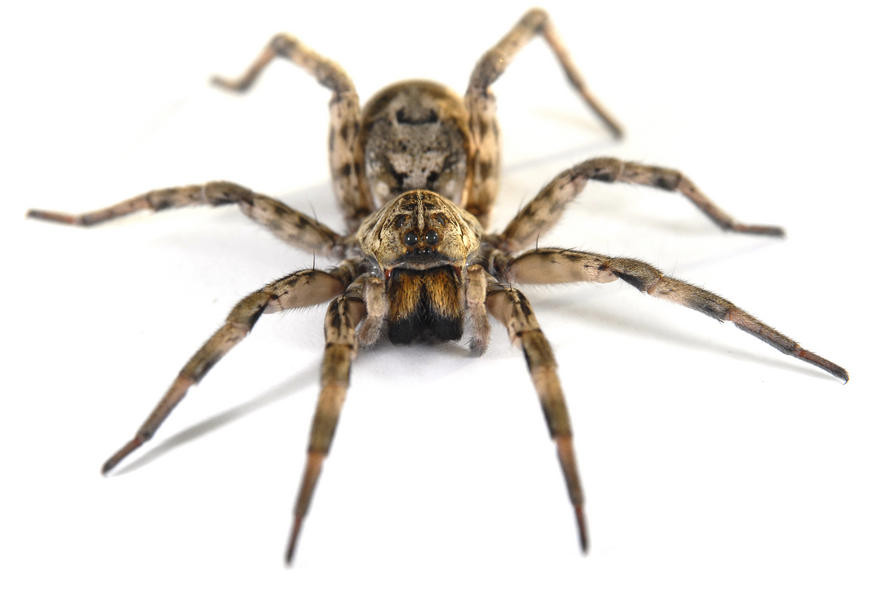
\includegraphics{wolf_spider.jpg}

\end{frame}



\begin{frame}
\frametitle{What is programming?}

\textbf{Definition:} \\$ $\\

\textit{Programming} is the art of instructing a computer to do exactly what you say through an \emph{algorithm}.\\$ $\\

\textbf{Definition:} \\$ $\\

\textit{Algorithms} are a process or set of rules to be followed in calculations or other problem-solving operations\\$ $\\

\end{frame}



\begin{frame}
\frametitle{Programming Defines the 21st Century Tool}

{\LARGE
``Humans are tool builders and we build tools that can dramatically amplify our innate human abilities. Of all of the inventions of humans, the computer is going to rank near if not at the top as history unfolds and we look back. And it is the most awesome tool that we have ever invented.''
}
\\$ $\\

-- Steve Jobs (from the \href{https://www.youtube.com/watch?v=_isT7GWplbs}{Lost Interview})

\end{frame}


\begin{frame}
\frametitle{Why study programming now?}
Programming has been available from the advent of computers. But, why am I hearing about it now?

\center{\Large{What's changed?}}
\flushleft

A shift from working within \textbf{excel} to \textbf{automation} \\

  \begin{columns}
    \begin{column}{.5\linewidth}
    \begin{center}
    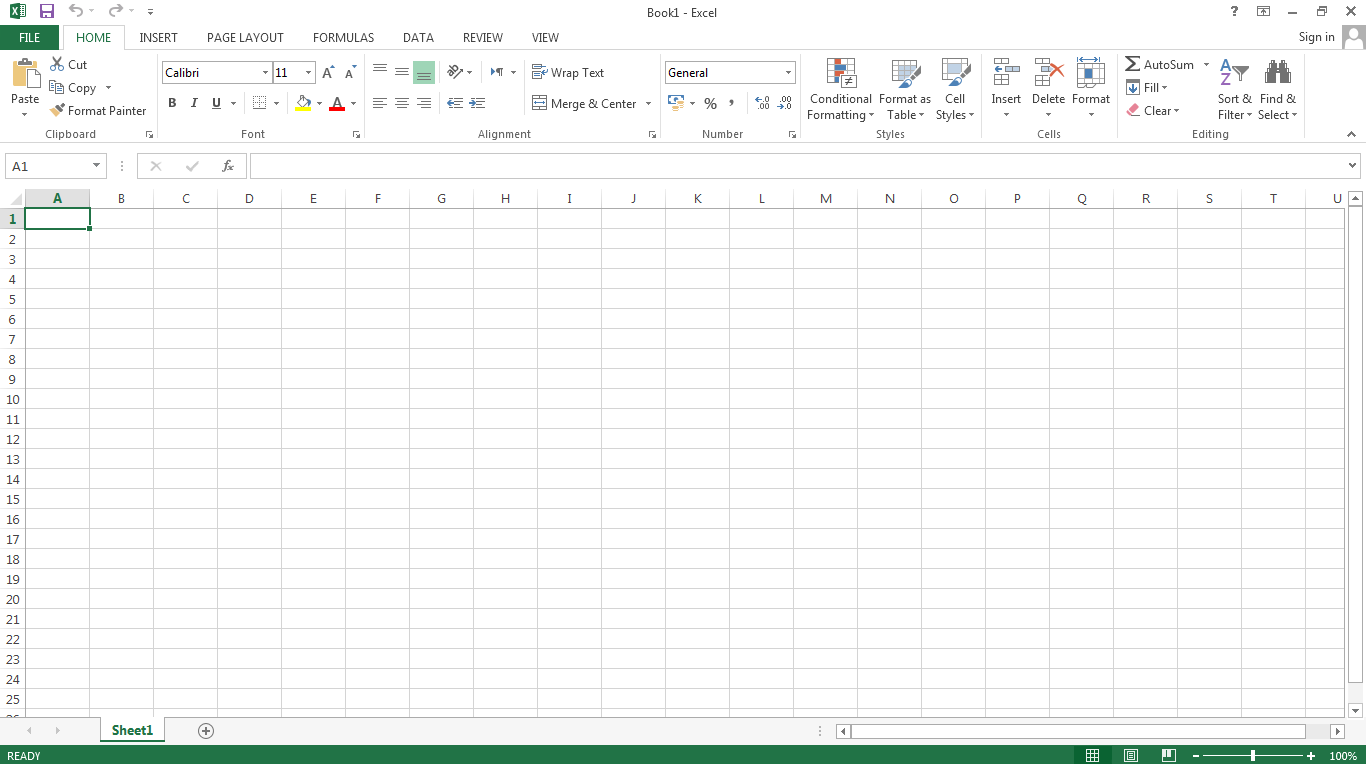
\includegraphics[scale=.15]{excel.png}
    \end{center}
    \end{column}
    \begin{column}{.5\linewidth}
    \begin{center}
    
\includegraphics[scale=.2]{phpCode.png}
    \end{center}
    \end{column}
  \end{columns}
$ $ \\
Plus, a lot more CPU power on a traditional desktop.
\end{frame}

\begin{frame}
\frametitle{Benefits}

The adoption of programming methods has several benefits:
\begin{enumerate}
\item Speed
\item Consistency
\item Resources
\item Computer Savviness
\item Logic
\end{enumerate}
\end{frame}


\section{Intro to R}


\begin{frame}
\frametitle{Learning a new language is HARD!}
\begin{center}
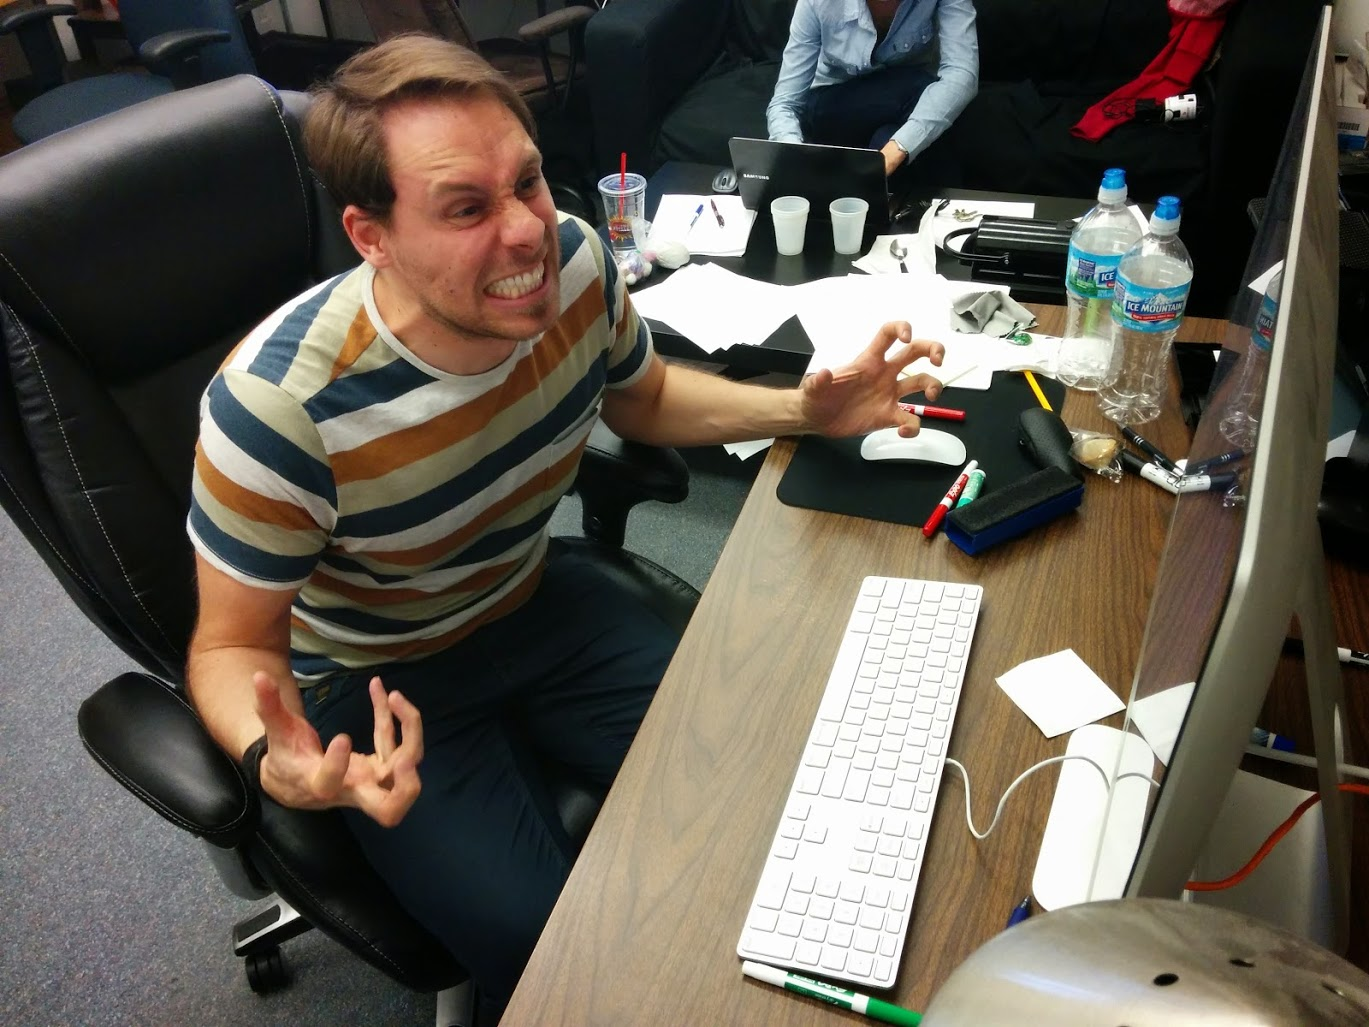
\includegraphics[height=7cm, width=12cm]{roberto_smash.jpg}
\end{center}
\end{frame}


\begin{frame}
\begin{center}
\Huge Ready?
\end{center}
\end{frame}


\subsection{Background of R}

\begin{frame}
\frametitle{What is R?}
\begin{itemize}
\item R is a language designed specifically for statistical computing and graphics
\item R is an interactive interface to many different tools.
\item R is based on the S language, which was developed by Bell laboratories
\item R is an open source (e.g. \textcolor{red}{free}) project that is cross platform (OS X, Windows, and Linux)
\item R is available on \textit{The R Project for Statistical Computing} website \href{http://www.r-project.org}{http://www.r-project.org}
\end{itemize}
\end{frame}

\begin{frame}
\frametitle{Why R?}
Pros:
\begin{itemize}
\item It's free!
\item Large repository of packages that often contain the latest breakthrough statistical methods
\item Able to integrate Fortran, C, C++, and Python code via wrappers
\item UIUC STAT Dept. Standard
\end{itemize}
Cons:
\begin{itemize}
\item Objects are always kept in RAM leading to Total System RAM constraining tasks
\item Pass by value (e.g. make a copy) quickly eats up available RAM
\item Very steep learning curve
\item Skin and bones UI
\end{itemize}
\end{frame}

\subsection{RStudio IDE}
\begin{frame}
\frametitle{RStudio}
RStudio is an Integrated Developer Environment (IDE) for R. 
\begin{itemize}
\item Advanced GUI that emphasizes a project workflow
\item Provides support for a novice user and an advanced user
\item Open source (e.g. \textcolor{red}{free}) project that is cross platform (OS X, Windows, and Linux)
\item Download RStudio via \href{http://www.rstudio.com/products/rstudio/download/}{http://www.rstudio.com}
\item OR use RStudio \url{https://rstudio.stat.illinois.edu}
\end{itemize}
\end{frame}

\begin{frame}
\frametitle{RStudio View}
\begin{center}
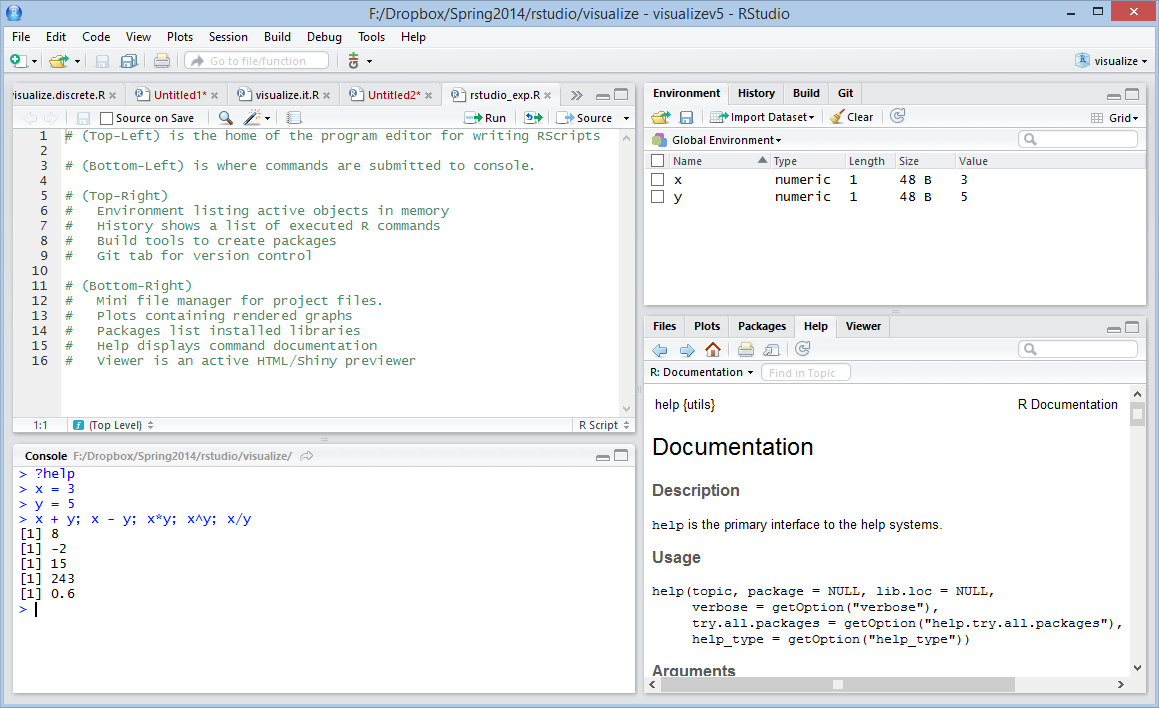
\includegraphics[scale=0.38]{rstudio_view.png}
\end{center}

\end{frame}

\begin{frame}[fragile]
\frametitle{Warming up to R}

To begin our exploration of the R language, we'll use R to mimic a scientific calculator. Scientific calculators are able to:

\begin{itemize}
\item Compute mathematical expressions.
\item Temporarily store values in a variable.
\end{itemize}

Explanations of the code, are given by comments predated by a  \#.
\\$ $\\
Output from the code is given by two \#\#. 
\end{frame}

\subsection{Sample Code}
\begin{frame}[fragile]
\frametitle{Storing Values and Calculations}
\begin{knitrout}
\definecolor{shadecolor}{rgb}{0.969, 0.969, 0.969}\color{fgcolor}\begin{kframe}
\begin{alltt}
\hlcom{# Create numeric object with values}
\hlstd{x} \hlkwb{=} \hlnum{3}
\hlstd{y} \hlkwb{=} \hlnum{5}

\hlcom{# Perform calculations}
\hlstd{x} \hlopt{+} \hlstd{y}
\end{alltt}
\begin{verbatim}
## [1] 8
\end{verbatim}
\begin{alltt}
\hlstd{x} \hlopt{-} \hlstd{y}
\end{alltt}
\begin{verbatim}
## [1] -2
\end{verbatim}
\begin{alltt}
\hlcom{# x*y; x/y; x^y;}
\end{alltt}
\end{kframe}
\end{knitrout}
\end{frame}

\begin{frame}[fragile]
\frametitle{Vectors}

In R, a number like \textbf{5} is treated as a vector, or a collection of values, with \textbf{length of 1}. 
\\$ $\\
We will see at a later time that this behavior, while odd, is actual pretty great to \emph{vectorize} computations.
\end{frame}

\begin{frame}[fragile]
\frametitle{Vectors}
\begin{knitrout}\small
\definecolor{shadecolor}{rgb}{0.969, 0.969, 0.969}\color{fgcolor}\begin{kframe}
\begin{alltt}
\hlstd{x} \hlkwb{=} \hlkwd{c}\hlstd{(}\hlnum{1}\hlstd{,}\hlnum{2}\hlstd{,}\hlnum{3}\hlstd{,}\hlnum{4}\hlstd{,}\hlnum{5}\hlstd{)} \hlcom{# Create vector}
\hlstd{y} \hlkwb{=} \hlnum{6}\hlopt{:}\hlnum{10}         \hlcom{# Shorthand}

\hlkwd{cbind}\hlstd{(x, y)}      \hlcom{# Combine Columns to form Matrix: 5 x 2}
\end{alltt}
\begin{verbatim}
##      x  y
## [1,] 1  6
## [2,] 2  7
## [3,] 3  8
## [4,] 4  9
## [5,] 5 10
\end{verbatim}
\begin{alltt}
\hlkwd{rbind}\hlstd{(x, y)}      \hlcom{# Combine Rows to form Matrix: 2 x 5}
\end{alltt}
\begin{verbatim}
##   [,1] [,2] [,3] [,4] [,5]
## x    1    2    3    4    5
## y    6    7    8    9   10
\end{verbatim}
\end{kframe}
\end{knitrout}
\end{frame}

\begin{frame}[fragile]
\frametitle{Built in Functions and Loops}

Like any good programming language before it, R has built in functions to aide in the workflow.
\\$ $\\ A small sampling of functions is:
\begin{itemize}
\item \texttt{sum} - Summation over elements $\sum\limits_{i = 1}^n {{x_i}}$
\item \texttt{mean} - Average over elements $\bar x = \frac{1}{n}\sum\limits_{i = 1}^n {{x_i}}$
\item \texttt{sd} - Standard Deviation over elements $\sqrt {\frac{1}{{n - 1}}\sum\limits_{i = 1}^n {{{\left( {{x_i} - \bar x} \right)}^2}} }$
\item \texttt{sample} - Random sample from ${x_1}, {x_2}, \ldots, {x_i}, \ldots, {x_n} $
\end{itemize}

$ $\\ To get help, use 
\begin{knitrout}
\definecolor{shadecolor}{rgb}{0.969, 0.969, 0.969}\color{fgcolor}\begin{kframe}
\begin{alltt}
\hlopt{?}\hlstd{function_name}
\end{alltt}
\end{kframe}
\end{knitrout}
\end{frame}

\begin{frame}[fragile]
\frametitle{Built-in Functions \& Loops}
\begin{knitrout}
\definecolor{shadecolor}{rgb}{0.969, 0.969, 0.969}\color{fgcolor}\begin{kframe}
\begin{alltt}
\hlstd{x} \hlkwb{=} \hlkwd{seq}\hlstd{(}\hlnum{1}\hlstd{,} \hlnum{10}\hlstd{,} \hlkwc{by} \hlstd{=} \hlnum{2}\hlstd{)}   \hlcom{# 1, 3, 5, 7, 9}
\hlstd{y} \hlkwb{=} \hlkwd{seq}\hlstd{(}\hlnum{10}\hlstd{,} \hlnum{30}\hlstd{,} \hlkwc{by} \hlstd{=} \hlnum{5}\hlstd{)}  \hlcom{# 10, 15, .. , 30}

\hlstd{result} \hlkwb{=} \hlkwd{numeric}\hlstd{(}\hlnum{1}\hlstd{)}      \hlcom{# Storage}
\hlkwa{for}\hlstd{(i} \hlkwa{in} \hlnum{1}\hlopt{:}\hlkwd{length}\hlstd{(x))\{}   \hlcom{# (variable in sequence)}
  \hlstd{result} \hlkwb{=} \hlstd{x[i]} \hlopt{+} \hlstd{result}
\hlstd{\}}                        \hlcom{# Loop (slow)}

\hlstd{(out} \hlkwb{=} \hlkwd{sum}\hlstd{(x))}           \hlcom{# Vectorized Function (faster)}
\end{alltt}
\begin{verbatim}
## [1] 25
\end{verbatim}
\begin{alltt}
\hlkwd{all.equal}\hlstd{(result, out)}   \hlcom{# Same value}
\end{alltt}
\begin{verbatim}
## [1] TRUE
\end{verbatim}
\begin{alltt}
\hlcom{#sd(x)                   # Standard Deviation}
\hlcom{#cor(x,y)                # Correlation}
\hlcom{#cov(x,y)                # Covariance}
\end{alltt}
\end{kframe}
\end{knitrout}
\end{frame}

\section{Types of Languages}

\begin{frame}
\frametitle{Talking to a Computer}

\begin{itemize}
\item In order to talk to a computer, you must speak its dialect. 
\item The dialect though is normally in 1's and 0's (or binary). 
\item Until \href{http://www.biography.com/people/grace-hopper-21406809}{Rear Admiral Grace M. Hopper} came along...
\end{itemize}

Now, we have the option of:

\begin{figure}
\centering
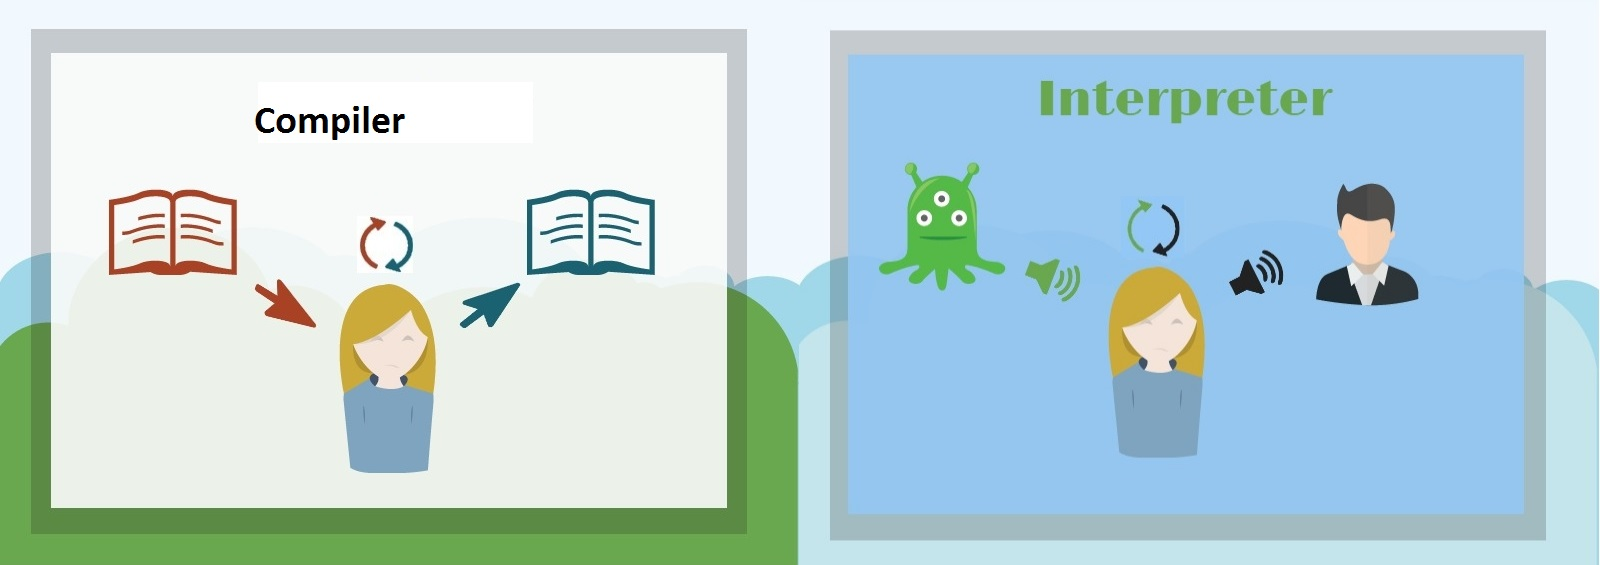
\includegraphics[width=\linewidth]{compiler_vs_interpreter}
\end{figure}

\end{frame}

\subsection{Interpreters}
\begin{frame}
\frametitle{What is an Interpreter?}

An \textit{interpreter} is a program that translates a high-level language into a low-level one, but it does it at the moment the program is run. 
\\$ $\\
So, the interpreter takes the source code, one line at a time, and translates each line before executing it. Every time the program runs.
\\$ $\\
Think of like a person providing a ``real time translation'' to a conversation.

\begin{center}

% Define block styles
\tikzstyle{decision} = [diamond, draw, fill=blue!20, 
    text width=4.5em, text badly centered, node distance=3cm, inner sep=0pt]
\tikzstyle{block} = [rectangle, draw, fill=blue!20, 
    text width=5em, text centered, rounded corners, minimum height=1cm]
\tikzstyle{line} = [draw, -latex']
\tikzstyle{cloud} = [draw, ellipse,fill=red!20, node distance=3cm,
    minimum height=2em]
    
\begin{tikzpicture}[node distance = 2cm, auto]
    % Place nodes
    \node [block, minimum height=3cm] (interpreter) {Interpreter};
    \node [cloud, align=center, left= of interpreter.north] (source) {Source \\ Code};
    \node [cloud, left= of interpreter.south] (input) {Input};
    \node [cloud, right= of interpreter.center] (output) {Output};
    % Draw edges
    \path [line] (source) -> (interpreter);
    \path [line] (input) -> (interpreter);
    \path [line] (interpreter) -> (output);
\end{tikzpicture}
\end{center}

\end{frame}

\begin{frame}[fragile]
\frametitle{Interpreters: Pros \& Cons}
As a result of the program being instantly translated, it is able to immediately provide feedback (e.g. output, errors, etc).\\$ $\\

For example, entering the following into R yields:
\begin{knitrout}
\definecolor{shadecolor}{rgb}{0.969, 0.969, 0.969}\color{fgcolor}\begin{kframe}
\begin{alltt}
\hlnum{3}\hlopt{+}\hlnum{4}
\end{alltt}
\begin{verbatim}
## [1] 7
\end{verbatim}
\end{kframe}
\end{knitrout}

The downside to this approach are:
\begin{enumerate}
\item The lack of optimized code 
\item Constant translation
\end{enumerate}

\end{frame}

\begin{frame}[fragile]
\frametitle{A looping example}
  \begin{columns}
    \begin{column}{.5\linewidth}
\begin{knitrout}
\definecolor{shadecolor}{rgb}{0.969, 0.969, 0.969}\color{fgcolor}\begin{kframe}
\begin{alltt}
\hlstd{bad.loop} \hlkwb{=} \hlkwa{function}\hlstd{()\{}
  \hlstd{sum} \hlkwb{=} \hlnum{0}
  \hlkwa{for}\hlstd{(i} \hlkwa{in} \hlnum{1}\hlopt{:}\hlnum{1000}\hlstd{)\{}
    \hlstd{a} \hlkwb{=} \hlnum{1}\hlopt{/}\hlkwd{sqrt}\hlstd{(}\hlnum{2}\hlstd{)} \hlcom{# In loop}
    \hlstd{sum} \hlkwb{=} \hlstd{(sum}\hlopt{+}\hlstd{i)}\hlopt{*}\hlstd{a}
  \hlstd{\}}
  \hlstd{sum}
\hlstd{\}}
\end{alltt}
\end{kframe}
\end{knitrout}
    \end{column}
    \begin{column}{.5\linewidth}
\begin{knitrout}
\definecolor{shadecolor}{rgb}{0.969, 0.969, 0.969}\color{fgcolor}\begin{kframe}
\begin{alltt}
\hlstd{good.loop} \hlkwb{=} \hlkwa{function}\hlstd{()\{}
  \hlstd{sum} \hlkwb{=} \hlnum{0}
  \hlstd{a} \hlkwb{=} \hlnum{1}\hlopt{/}\hlkwd{sqrt}\hlstd{(}\hlnum{2}\hlstd{)} \hlcom{# Out of Loop}
  \hlkwa{for}\hlstd{(i} \hlkwa{in} \hlnum{1}\hlopt{:}\hlnum{1000}\hlstd{)\{}
    \hlstd{sum} \hlkwb{=} \hlstd{(sum}\hlopt{+}\hlstd{i)}\hlopt{*}\hlstd{a}
  \hlstd{\}}
  \hlstd{sum}
\hlstd{\}}
\end{alltt}
\end{kframe}
\end{knitrout}
    \end{column}
  \end{columns}

\begin{center}
\begin{knitrout}
\definecolor{shadecolor}{rgb}{0.969, 0.969, 0.969}\color{fgcolor}
\begin{tabular}{l|r|r|r|r|r}
\hline
test & replications & elapsed & relative & user.self & sys.self\\
\hline
good.loop() & 100 & 0.045 & 1.000 & 0.041 & 0.003\\
\hline
bad.loop() & 100 & 0.059 & 1.311 & 0.057 & 0.001\\
\hline
\end{tabular}


\end{knitrout}
\end{center}
\end{frame}

\subsection{Compilers}
\begin{frame}[fragile]
\frametitle{What is a Compiler? Can it do my taxes?}

A compiler takes source code tries to optimize it before converting it into machine language \textbf{once}. After it is done compiling, the code can then be ran again and again without ever needing to be recompiled.\\$ $\\

So, a compiler is like an editor who is asked to look over a paper. If it thinks something can be better, then it will take the initiative and implement that option.\\$ $\\

\begin{center}
% Define block styles
\tikzstyle{block} = [rectangle, draw, fill=blue!20, 
    text width=5em, node distance=1cm, rounded corners, minimum height=1cm]
\tikzstyle{line} = [draw, -latex']
\tikzstyle{cloud} = [draw, ellipse,fill=red!20, node distance=1cm,
    minimum height=2em]
    
\begin{tikzpicture}[node distance = 2cm, auto]
    % Place nodes
    \node [cloud, align=center] (source) {Source \\ Code};
    \node [block, right=of source] (compiler) {Compiler};
    \node [cloud, align=center, right= of compiler] (machine) {Machine \\ Code};
    \node [cloud, below= of source] (input) {Input};
    \node [block, align=center, right= of input] (execute) {Executable \\ Program};
    \node [cloud, right= of execute] (output) {Output};
    % Draw edges
    \path [line] (source) -> (compiler);
    \path [line] (compiler) -> (machine);
    \path [line] (input) -> (execute);
    \path [line] (execute) -> (output);

    \path [line] (machine) -> (execute.north);
\end{tikzpicture}

\end{center}

\end{frame}

\begin{frame}[fragile]
\frametitle{Compilers: Pros}
Compilers will attempt to optimize the code that they are given.\\$ $\\
After succesful compiled, code will not need to be compiled again*.\\$ $\\

  \begin{columns}
    \begin{column}{.4\linewidth}
    {\textbf{Base R}}
\begin{knitrout}\tiny
\definecolor{shadecolor}{rgb}{0.969, 0.969, 0.969}\color{fgcolor}\begin{kframe}
\begin{alltt}
\hlstd{good.loop} \hlkwb{=} \hlkwa{function}\hlstd{()\{}
  \hlstd{sum} \hlkwb{=} \hlnum{0}
  \hlstd{a} \hlkwb{=} \hlnum{1}\hlopt{/}\hlkwd{sqrt}\hlstd{(}\hlnum{2}\hlstd{)} \hlcom{# Out of Loop}
  \hlkwa{for}\hlstd{(i} \hlkwa{in} \hlnum{1}\hlopt{:}\hlnum{1000}\hlstd{)\{}
    \hlstd{sum} \hlkwb{=} \hlstd{(sum}\hlopt{+}\hlstd{i)}\hlopt{*}\hlstd{a}
  \hlstd{\}}
  \hlstd{sum}
\hlstd{\}}
\end{alltt}
\end{kframe}
\end{knitrout}
    \end{column}
    \begin{column}{.6\linewidth}
     {\textbf{Bytecompiled R}}
\begin{knitrout}\tiny
\definecolor{shadecolor}{rgb}{0.969, 0.969, 0.969}\color{fgcolor}\begin{kframe}
\begin{verbatim}
## list(.Code, list(8L, LDCONST.OP, 1L, SETVAR.OP, 2L, POP.OP, LDCONST.OP, 
##     3L, GETFUN.OP, 4L, PUSHCONSTARG.OP, 5L, CALL.OP, 6L, DIV.OP, 
##     7L, SETVAR.OP, 8L, POP.OP, LDCONST.OP, 3L, LDCONST.OP, 9L, 
##     COLON.OP, 10L, STARTFOR.OP, 12L, 11L, 42L, GETVAR.OP, 2L, 
##     GETVAR.OP, 11L, ADD.OP, 13L, GETVAR.OP, 8L, MUL.OP, 14L, 
##     SETVAR.OP, 2L, POP.OP, STEPFOR.OP, 29L, ENDFOR.OP, POP.OP, 
##     GETVAR.OP, 2L, RETURN.OP), list({
##     sum = 0
##     a = 1/sqrt(2)
##     for (i in 1:1000) {
##         sum = (sum + i) * a
##     }
##     sum
## }, 0, sum, 1, sqrt, 2, sqrt(2), 1/sqrt(2), a, 1000, 1:1000, i, 
##     for (i in 1:1000) {
##         sum = (sum + i) * a
##     }, sum + i, (sum + i) * a))
\end{verbatim}
\end{kframe}
\end{knitrout}
    \end{column}
  \end{columns}
\end{frame}

\begin{frame}[fragile]
\frametitle{Compilers: Cons}

Compilers spend a lot of time analyzing and processing the program.\\$ $\\

They require the \textbf{ENTIRE} program to be sent.\\$ $\\

There is additional storage required to handle the machine generated code.\\$ $\\

Errors will only appear \textbf{AFTER} the entire program is analyzed.\\$ $\\

Did I mention compilers take a lot of time?

\end{frame}

\begin{frame}[fragile]
\frametitle{A looping example redux}
After applying a compiler, there should be a noticeable change...
\begin{knitrout}
\definecolor{shadecolor}{rgb}{0.969, 0.969, 0.969}\color{fgcolor}\begin{kframe}
\begin{alltt}
\hlkwd{library}\hlstd{(}\hlstr{"compiler"}\hlstd{)}
\hlstd{good.comp} \hlkwb{=} \hlkwd{cmpfun}\hlstd{(good.loop)}
\hlstd{bad.comp} \hlkwb{=} \hlkwd{cmpfun}\hlstd{(bad.loop)}
\end{alltt}
\end{kframe}
\end{knitrout}

\begin{center}
\begin{knitrout}
\definecolor{shadecolor}{rgb}{0.969, 0.969, 0.969}\color{fgcolor}
\begin{tabular}{l|r|r|r|r|r}
\hline
test & replications & elapsed & relative & user.self & sys.self\\
\hline
good.comp & 100 & 0.007 & 1.000 & 0.007 & 0.000\\
\hline
bad.comp & 100 & 0.020 & 2.857 & 0.019 & 0.001\\
\hline
good.loop & 100 & 0.039 & 5.571 & 0.035 & 0.001\\
\hline
bad.loop & 100 & 0.057 & 8.143 & 0.054 & 0.001\\
\hline
\end{tabular}


\end{knitrout}
\end{center}
\end{frame}

\begin{frame}
\frametitle{To summarize..}
  \begin{columns}
    \begin{column}{.5\linewidth}
\textbf{Compilers}
Pros:
\begin{enumerate}
  \item Code is optimized.
  \item Program runs really fast... (Vroom Vroom fast)
  \item Compiles once.*
  \item Conditional statements are faster
\end{enumerate}
Cons:
\begin{enumerate}
  \item Lots of time spent analyzing and optimizing code
  \item More storage required due to machine code.
  \item Errors only show at the end
\end{enumerate}
    \end{column}
    \begin{column}{.5\linewidth}
\textbf{Interpreters}
Pros:
\begin{enumerate}
  \item Immediate Feedback
  \item Less storage required
  \item Friendlier
\end{enumerate}
Cons:
\begin{enumerate}
  \item Takes single instruction as input.
  \item Constant compiles from high-level to low-level
  \item Slow program execution
  \item Conditional statements are slower.
\end{enumerate}
    \end{column}
  \end{columns}
  
\flushright *no errors, changes, etc.

\end{frame}



\begin{frame}
\frametitle{Questions? Comments?}

\centering
\Huge
James Balamuta
\href{mailto:balamut2@illinois.edu}{\nolinkurl{balamut2@illinois.edu} }
\href{http://stat385.thecoatlessprofessor.com}{stat385.thecoatlessprofessor.com}


\end{frame}

\end{document}
